% Enable warnings about problematic code
\RequirePackage[l2tabu, orthodox]{nag}

\documentclass{WeSTassignment}

% The lecture title, e.g. "Web Information Retrieval".
\lecture{Introduction to Web Science}
% The names of the lecturer and the instructor(s)
\author{%
  Prof. Dr.~Steffen~Staab\\{\normalsize\mailto{staab@uni-koblenz.de}} \and
  Ren{\'e}~Pickhardt\\{\normalsize\mailto{rpickhardt@uni-koblenz.de}} \and
   Korok~Sengupta\\{\normalsize\mailto{koroksengupta@uni-koblenz.de}}
}
% Assignment number.
\assignmentnumber{3}
% Institute of lecture.
\institute{%
  Institute of Web Science and Technologies\\%
  Department of Computer Science\\%
  University of Luxembourg%
}
% Date until students should submit their solutions.
\datesubmission{November 16, 2016, 10:00 a.m.}
% Date on which the assignments will be discussed in the tutorial.
\datetutorial{November 18, 2016, 12:00 p.m.}

% Set langauge of text.
\setdefaultlanguage[
  variant = american, % Use American instead of Britsh English.
]{english}

% Specify bib file location.
\addbibresource{bibliography.bib}

% For left aligned centerd boxes
% see http://tex.stackexchange.com/a/25591/75225
\usepackage{varwidth}
\usepackage{listings}

% ==============================================================================
% Document

\begin{document}

\maketitle

The main objective of this assignment is for you understand different concepts that are associated with the "Web". In this assignment we cover two topics: 1) DNS \& 2) Internet. 

These tasks are not always specific to \enquote{Introduction to Web Science}.
For all the assignment questions that require you to write a code, make sure to include the code in the answer sheet, along with a separate python file. Where screen shots are required, please add them in the answers directly and not as separate files.\\ \\ 

%Please mention your team Names here: 
Team Name: hotel

% ------------------------------------------------------------------------------

\section{DIG Deeper (5 Points)}

Assignment 1 started with you googling certain basic tools and one of them was "\emph{dig}". 
\begin{enumerate}
\item Now using that dig command, find the IP address of \url{ www.uni-koblenz-landau.de}
\item In the result, you will find "SOA". What is SOA? 
\item Copy the SOA record that you find in your answer sheet and explain each of the components of SOA with regards to your find. Merely integrating answers from the internet wont fetch you points.  

\end{enumerate}
Try the experiment once from University network and once from Home network and see if you can find any differences and if so, clarify why. 

\textbf{Answers:}\\

% ------------------------------------------------------------------------------

\section{Exploring DNS (10 Points)}

In the first part of this assignment you were asked to develop a simple TCP Client Server. Now, using \textbf{that} client server setup.
This time a url should be send to the server and the server will split the url into the following:\\ 

\url{http://www.example.com:80/path/to/myfile.html?key1=value1&key2=value2#InTheDocument}

\begin{enumerate}
\item Protocol
\item Domain
\item Sub-Domain
\item Port number
\item Path
\item Parameters
\item Fragment
\end{enumerate}

The Protocol for sending the URL will be a string terminated with \backslash r \backslash n.

P.S.: You are \textbf{not} allowed to use libraries like \texttt{urlparse} for this question. You will also not use "Regular Expressions" for this. 

\textbf{Answer:} \\
\underline{Server:}\\
\lstinputlisting{server.py}
\underline{client:}\\
\lstinputlisting{client.py}


% ------------------------------------------------------------------------------


\section{DNS Recursive Query Resolving (5 Points)}

You have solved the "Routing Table" question in Assignment 2. We updated the routing tables once more. resulting in the following tables creating the following topology 

% Please add the following required packages to your document preamble:
% \usepackage[normalem]{ulem}
% \useunder{\uline}{\ul}{}
\begin{table}[h]
\centering
\caption{Routing Table}
\label{routing table}
\scalebox{0.8}{
\begin{tabular}{|c|c|c|c|c|c|c|c|c|c|c|}
\hline
\multicolumn{3}{|c|}{\textbf{Router1}} &        & \multicolumn{3}{c|}{\textbf{Router2}} &        & \multicolumn{3}{c|}{\textbf{Router3}} \\ \hline
Destination  & Next Hop    & Interface &        & Destination & Next Hop    & Interface &        & Destination  & Next Hop   & Interface \\ \hline
67.0.0.0     & 67.68.3.1   & eth 0     &        & 205.30.7.0  & 205.30.7.1  & eth 0     &        & 205.30.7.0   & 205.30.7.2 & eth 0     \\ \hline
62.0.0.0     & 62.4.31.7   & eth 1     &        & 156.3.0.0   & 156.3.0.6   & eth 1     &        & 88.0.0.0     & 88.6.32.1  & eth 1     \\ \hline
88.0.0.0     & 88.4.32.6   & eth 2     &        & 26.0.0.0    & 26.3.2.1    & eth 2     &        & 25.0.0.0     & 25.03.1.2  & eth 2     \\ \hline
141.71.0.0   & 141.71.20.1 & eth 3     &        & 141.71.0.0  & 141.71.26.3 & eth 3     &        & 121.0.0.0    & 121.0.3.1  & eth 3     \\ \hline
26.0.0.0     & 141.71.26.3 & eth3      &        & 67.0.0.0    & 141.71.20.1 & eth 3     &        & 156.3.0.0    & 205.30.7.1 & eth 0     \\ \hline
156.3.0.0    & 88.6.32.1   & eth 2     &        & 62.0.0.0    & 141.71.20.1 & eth 3     &        & 26.0.0.0     & 205.30.7.1 & eth 0     \\ \hline
205.30.7.0   & 141.71.26.3 & eth 3     &        & 88.0.0.0    & 141.71.20.1 & eth 3     &        & 141.71.0.0   & 205.30.7.1 & eth 0     \\ \hline
25.0.0.0     & 88.6.32.1   & eth 2     &        & 25.0.0.0    & 205.30.7.2  & eth 0     &        & 67.0.0.0     & 88.4.32.6  & eth 1     \\ \hline
121.0.0.0    & 88.6.32.1   & eth 2     &        & 121.0.0.0   & 205.30.7.2  & eth 0     &        & 62.0.0.0     & 88.4.32.6  & eth 1     \\ \hline
\end{tabular}
}
\end{table}

\begin{figure}[h]
  \centering
  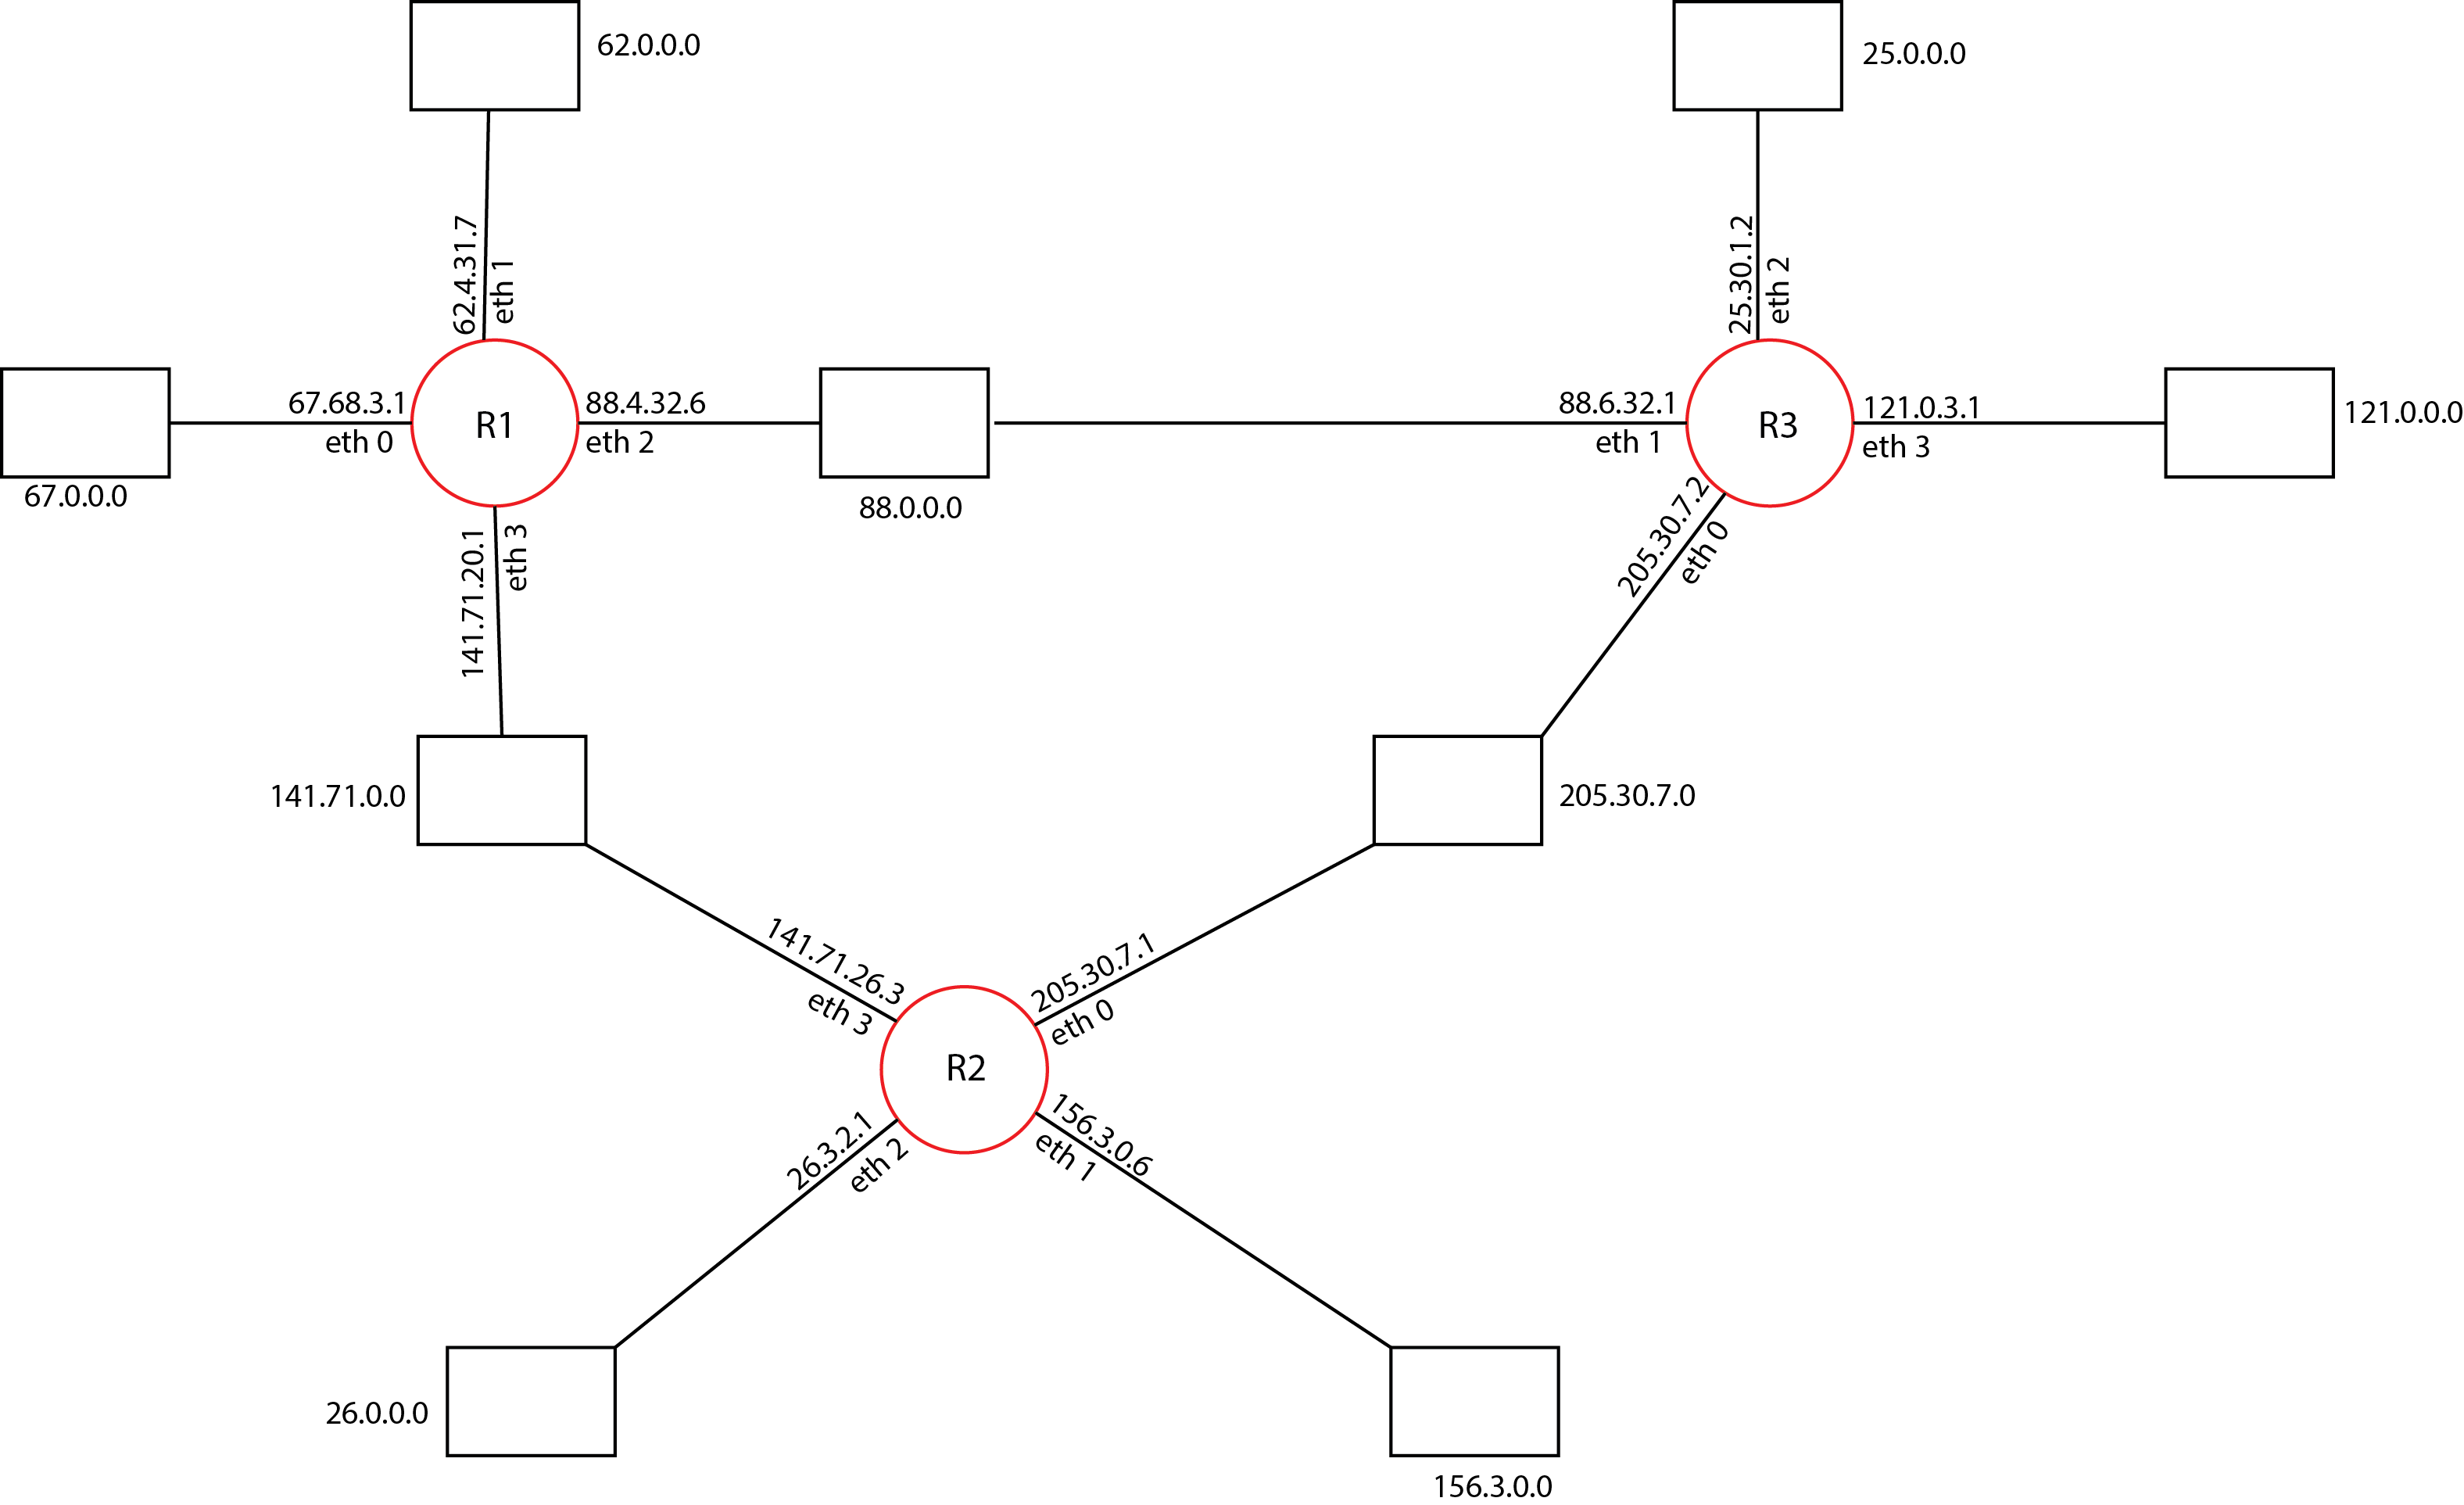
\includegraphics[scale=0.45]{ass3_DNS.png}
   \caption{DNS Routing Network}
     \label{fig:routing} 
\end{figure}

Let us asume a client with the following ip address 67.4.5.2 wants to resolve the following domain  \texttt{subdomain.webscienceexampledomain.com} using the DNS.

You can further assume the root name server has the IP address of 25.8.2.1 and the name-server for \texttt{webscienceexampledomain.com} has the IP address 156.3.20.2. 
Finally the sub-domain is handled by a name server with the IP of 26.155.36.7. 

Please explain how the traffic flows through the network in order to resolve the recursive DNS query. You can assume ARP tables are cached so that no ARP-requests have to be made. 

\textbf{Answer}: \\
We assume the DNS Server for the client is the router of the network, in this case Router 1.\\
\\
67.4.5.2 creates an IP packet with the source address 67.4.5.2 and destination address 67.68.3.1 (Router 1). Inside there is the DNS request. This IP packet is send as an ethernet frame to 67.68.3.1. 
67.68.3.1 receives the frame and forwards the encapsulated IP packet to 88.6.32.1 which sends the packet to the root name server 25.8.2.1.\\
\\
The root name server creates an IP packet with the source address 25.8.2.1 and the destination address 67.68.3.1.\\
Inside there is the DNS response which tells the DNS Server (Router 1) to send its request to the nameserver responsible for the webscienceexampledomain.com. zone and the IP address for said nameserver (156.3.20.2).\\
This IP packet is send as an ethernet frame to 25.30.1.2. 25.30.1.2 receives the frame and forwards the encapsulated IP packet to Router 1 / the DNS Server at 88.4.32.6.\\
\\
Router 1 creates an IP packet with the source address 141.71.20.1 and the destination address 156.3.20.2. Inside there is the DNS request from the client. This IP packet is send as an ethernet frame to 141.71.26.3. 141.71.26.3 receives the frame and forwards the encapsulated IP packet to the nameserver at 156.3.20.2.\\
156.3.20.2 creates an IP packet with the source address 156.3.20.2 and the destination address 67.68.3.1. Inside there is the DNS response  which tells the DNS Server (Router 1) to send its request to the nameserver responsible for the subdomain.webscienceexampledomain.com. zone and the IP address for said nameserver (26.155.36.7).\\
This IP packet is send as an ethernet frame to 156.3.0.6. 156.3.0.6 receives the frame and forwards the encapsulated IP packet to Router 1 at 141.71.20.1.\\
\\
Router 1 creates an IP packet with the source address 141.71.20.1 and the destination address 26.155.36.7. Inside there is the DNS request. This packet is send as an ethernet frame to 141.71.26.3. 141.71.26.3 receives the packet and forwards the encapsulated IP packet to 26.155.36.7.\\
26.155.36.7 creates an IP packet with the source address 26.155.36.7 and the destination address 141.71.20.1. Inside there is the DNS response including the IP address of the requested domain.\\
 This packet is send as an ethernet frame to 26.3.2.1. 26.3.2.1 receives the frame and forwards the encapsulated IP packet to 141.71.20.1.\\
\\
Router 1 caches the IP address of the DNS request for future requests and creates an IP packet with the source address 67.68.3.1 and the destination address 67.4.5.2. Inside there is the DNS response including the requested IP address. The IP packet is send as an ethernet frame to 67.4.5.2. 67.4.5.2 receives the frame and now knows the IP address of subdomain.webscienceexample.com





% ------------------------------------------------------------------------------




\makefooter

\end{document}
